This document concludes the 12th HGSFP Winter School that took place at
the University Center in Obergurgl from 16th to 20th of January 2019. In
total, 52 graduate students from Heidelberg and 10 lecturers participated
in the five-day event. The aim of the Winter School was to give students
the opportunity to get insights into other research fields in
Heidelberg apart from their own field. In the course of this, one of the
focal points was the scientific exchange between the students
themselves and students and lecturers in a friendly atmosphere. To this
end, we organized a scientific programme consisting of 10 lectures given
by speakers from Heidelberg and other universities and two poster
sessions with elevator talks (see Appendix A).


\section*{Participant Selection}
As expected, we received more applications for the school than spots were available. We therefore had to select participants from the pool of applicants, which we wanted to perform as fair as possible. We felt it was important to be both transparent about and accountable for our selection. For this reason, we imposed a selection algorithm, laid open the complete procedure (with anonymized data)\footnote{https://github.com/matiscke/HGSFPschoolParticipantSelection}, and explain what decisions went into the selection. In the following, we give an overview on how we selected the participants for the HGSFP winter school 2019.

\subsection*{Asking The Right Questions}
Designing the application form was perhaps the most difficult task, and it is at this stage that conference organizers will already want to put serious thought into the goals of the workshop and the ideal mix of participants to achieve those goals. It should be obvious, but you will only be able to include categories in your selection that you actually ask for.

\subsection*{Pre-selection}
Excluding speakers, we have 52 spots for the meeting. Our participant selection proceeded in two parts. In the first part, we rejected candidates outright who were either (1) duplicate entries or (2) candidates who had informed us that they would not be able to come. Two spots were reserved for the HGSFP representatives. Finally, we pre-selected the organizing committee, who needs to be present at the school. Thus, a total of 8 participants (6 organizers, 2 representatives) were pre-selected. We then anonymized our applicant pool by replacing names and other identifying information with a unique identifier. 

For the remaining 52 - 8 = 44 slots, we used the software \texttt{entrofy} to optimize our participant set based on a set of well-defined criteria on which the organizers agreed. It's worth noting here that this discussion took place before performing the selection, which then depended entirely on the goals for the selection and was independent of the input data set. 

\subsection*{Target Distributions}
The targets define the fraction of participants in the final output set who share the same value of a property (e.g. 25\% of participants should be affiliated with the HGSFP branch "Fundamental Interactions and Cosmology"). The target fractions must sum up to be smaller or equal to 1.0 for each category. If the target fractions sum to a value smaller than one, the algorithm will try to fill up categories to at least the given fractions, and will ignore that category for the rest of the optimization procedure. The resulting mix of participants in the final set for this category will thus be a combination of the input fractions and the distribution in the input sample, conditioned on the constraints set by the remaining categories. Below, we will go through each category one by one and lay out our reasoning for the categories chosen. The justification for our choices is an abbreviated version of a longer discussion the organizing committee had before starting the selection procedure. We should note at this point that there is no "correct" way to choose target fractions; the target fractions must necessarily always be a function of the objectives and goals of the workshop, as defined by the organizers.

\subsection*{Selection Goals}
Broadly, the goals we defined for the HGSFP Winter School 2019 for participant selection are the following:
\begin{itemize}
	\item enable every HGSFP student to attend one winter school during their PhD:
	\begin{itemize}
		\item[$\Rightarrow$] strongly favor applicants that have not attended a HGSFP winter school before
		\item[$\Rightarrow$] favor applicants that are longer into their PhD (since the clock is ticking...)
	\end{itemize}
	\item Reflect the student numbers of the different HGSFP branches
	\item Increase the participation of underrepresented minorities (in our case this translates to an effort for gender equality)
\end{itemize}
~\\
\textbf{HGSFP branch}\\
For the branch attribute, we aim to reflect the distribution of the overall branch affiliation

~\\
\textbf{Previous Winter School Attendance}\\
Derived from our top requirement, the acceptance of applicants with previous attendance of a winter school should be an exception. We decided if we allow previous attendees at all based on the oversubscription of the school. The latter was not very high, we therefore decided to accept applicants with previous attendence only via the waiting list. We enforce this criterion further below and do not solve for this parameter.

~\\
\textbf{Gender Identity}\\
Any social engineering involving gender is necessarily subject to scrutiny. Our choices here reflect our beliefs about what we would like the Winter School to be: We recognize that underrepresented minorities are particularly underrepresented in physics, which is reflected in the number of non-male PhD students. We also recognize studies that show that diverse groups outperform groups lacking diversity among several axes. Representation is important: we believe that minority participants might feel more comfortable participating if they do not feel singled out based on their gender.

Realizing that an equal representation of genders cannot be realized given the input set, we choose to set a goal fraction of female participants slightly higher than the corresponding share in the HGSFP and allow a sufficient margin for the option "Don't identify with either".

~\\
\textbf{PhD Duration}\\
We aimed to give senior PhD students that have not participated in a Winter School before an advantage in the selection, since they have less or no opportunities to re-apply next year.

~\\
Aside from the organizers and representatives, the entire procedure was performed entirely without names and based only on the candidates' responses and the complex optimization of the participant selection with respect to our goals. After the selection, all applicants were informed about the outcome and applicants in the 'accepted' list were asked to confirm their attendance within a specified period. Not all participants accepted our invitation on the first round. Free spots were filled with applicants from the waiting list on a first-come, first-served basis with regard to our notification emails. 

~\\
More detailed information about our selection procedure and an interactive Jupyter notebook that includes the original code can be found on\\
https://github.com/matiscke/HGSFPschoolParticipantSelection.








\section*{Lectures}
We selected the lecturers based on a few key ideas: First, we tried to give the participants a glimpse of the wide range of different research areas within the HGSFP by selecting lecturers from very different research backgrounds both in experimental and theoretical physics. Furthermore, we asked lecturers at different stages of their academic career, from post-doctoral researcher to senior professor, to join the winter school, in order to encourage discussions between participants and lecturers on career choices in academia. Finally, we asked that all lecturers actively participate in the winter school in excess to their own lectures, in particular to allow for discussions with the participants in a relaxed atmosphere between lectures.
Each lecturer gave two lectures of 90 minutes each, with three lectures taking place in parallel such that the participants were able to choose a schedule of lectures according to their own interests. All lectures were structured in a way that also participants from different research fields could join. This opportunity to get a broader overview of the research activities within the HGSFP was embraced by the students. The combination of a high quality of lectures with a mixed, but interested audience lead to many discussions and exchanges of ideas during and also after the lectures.
In addition to the regular schedule of lectures there was a special lecture for all participants on the topic of avalanche research. The special lecture was accompanied by an excursion the following day, where the participants were able to gain some insight into the practical aspects of avalanche research and risk assessment.

\section*{Poster Sessions}
In addition to the lectures, the participants were asked to present their own research in form of a poster. There were two poster sessions on two of the evenings. We adopted the idea of previous years to start off the poster sessions by one minute-long ‘elevator talks’. Here, all students presenting their research in the given poster session had the opportunity to introduce themselves and the topic of their poster within one minute. This helped the participants to get an overview of potentially interesting posters. The poster sessions were well received by the students which expressed itself in particular in the lively discussions during the poster sessions and in particular also afterwards.

\section*{Venue}
The conference center of the university of Innsbruck was a perfect choice for the school. With all the participants and lecturers staying in the same place, the possibility to talk to other participants and lecturers was greatly enhanced. There were different rooms for all possible needs available, ranging from big lecture halls for the special lecture and the poster sessions, to smaller lecture halls, rooms for concentrated working as well as lounge areas for more relaxed discussions. A wide range of (sports) activities was available in the direct vicinity of the conference center. The staff of the conference center were very helpful in all situations, making the stay a very pleasant experience.


\section*{Travel}
Similar as in previous years, the travel was done by bus over night with two drivers, which allowed them to drive without the need for stops or a hotel room in Obergurgl,
as they could directly drive the way back. This allowed us to be in Obergurgl in time for breakfast. While it seemed exhausting for some people, as they arrival day did not have a 
fixed schedule and could be spent relaxing in the hotel, overall the participants where happy with this itinerary.
Traveling back was done on the late afternoon, giving everyone the time to enjoy the last afternoon while arriving in Heidelberg just before 11 pm. Following the general mood, a similar itinerary schedule is recommended for the future.

\section*{Social Event}
As a yearly tradition, the first evening of the Winter School was
devoted to the social event — Eisstockschiessen. The event served well for people to get to know each other in a relaxed and fun environment. The scope of the event seemed to be appreciated with everyone joining.
The last day was concluded with a big group going sledding which approximated a second social event, 
with less organizing and no funding, but being appreciated just as well.

\section*{Science Quiz}
This year we organized a Science Quiz as an additional social event.
Because this event was not in the program before the winter school, we regarded it as an additional, not mandatory event.
Still, all the students and speaker participated enthusiastically.
The participants formed teams and answered question from diverse topics ranging from fun facts about science to recent Nobel prizes.
According to the survey and the atmosphere during the event the science quiz was a definitive success.
The quiz itself did not cause any additional costs in the budget, because the rooms were booked for us because of the lectures and the prizes were merchandising articles from research projects at the Heidelberg University.

\newpage

\section{Lecture Abstracts}

\begin{center}
{{\large\bfseries Building Planets - A Journey along 40 Orders of Magnitude}\par} \medskip

{\large Til Brinstiel, Ludwig-Maximilians-Universität München\par}
\end{center}

\noindent Building planets is a dirty business. First of all, planets are made out of the dirt we call interstellar dust. Secondly, the physics involved is not "clean" in a sense that neither the processes involved, nor the initial conditions are known. Solid state physics, radiation transport, gas phase and surface chemistry, magnetic fields and hydrodynamic instabilities at high Reynolds numbers are just some of the aspects that are certainly involved in growing the sub-micrometer sized interstellar dust by 40 orders of magnitude in mass to a full-fledged planet. Given this complexity and dynamic range, it is perhaps not surprising, that the formation processes of planets are still poorly understood, even though thousands of planets beyond our solar system are known today.

Some of the biggest mysteries of planet formation lie in the early stages: growing the asteroid-sized building blocks of planets. Recent years have seen a revolution in observing capabilities at various wavelength ranges delivering data of unprecedented detail and sensitivity. They have partially confirmed our theoretical expectations, partially surprised us. In this lecture, I will discuss some of the basic concepts and the problems we are facing from the theoretical side. I will outline how they might be overcome and will show how recent observational break-throughs revoluzionize this exciting field, bringing us closer to solving the puzzle of planet formation.\par
\newpage


\begin{center}
{{\large\bfseries Galaxy Formation and Cosmology}\par} \medskip

{\large Tobias Buck, Max-Planck-Institut for Astronomy (MPIA), Heidelberg\par}
\end{center}

\noindent In these two lectures I will give a broad overview over the field of galaxy formation and evolution and the cosmological standard model.
Cosmology governs the evolution of the spacetime of our Universe. Thus, I will first discuss the reasoning and implications of the cosmological model and highlight our understanding about nucleosynthesis and structure formation within this model.
I will then move to describe the collection of observational facts about the galaxy population of our Universe in order to discuss the physical principles needed to explain these observations. Finally, I will briefly summarise current efforts and models in numerical galaxy formation to test physical mechanisms involved in the formation of galaxies.
 
\par
\newpage




\begin{center}
{{\large\bfseries Strongly Coupled Systems and the Applied Physics of Black Holes}\par} \medskip

{\large Carlo Ewerz, Institute for Theoretical Physics, Heidelberg University\par}
\end{center}

\noindent One of the most surprising findings of string theory is that quantum field theories and higher-dimensional gravity are closely connected, and can in fact be different descriptions of the same fundamental laws. The corresponding holographic dualities improve our understanding of fundamental theories of Nature and have many applications. In particular, they offer new and revolutionary insights into the behavior of strongly coupled quantum systems by connecting them to the physics of black holes. This has helped to discover universal behavior in many strongly coupled systems.
 
In the first part of the lecture, I will give a basic introduction to the principle of holographic duality. In the second part, I will present some examples and applications including the description of heavy quarks in a quark-gluon plasma and turbulence in a superfluid.
 
The lecture will start from basic (mostly undergraduate level) physics and does not require any expert knowledge of string theory etc.
\par
\newpage

\begin{center}
{{\large\bfseries Prospects and challenges of quantum computing}\par} \medskip

{\large Martin Gärttner, Kirchhoff-Institute for Physics, Heidelberg University\par}
\end{center}

\noindent “The first fusion reactor will be producing energy within 30 years from now.” This statement seems to be true independent of when it is made. Similarly, the Wikipedia page on quantum computing has been stating for quite a while now “the development of actual quantum computers is still in its infancy”. Will this statement ever be removed? The massive investments into quantum technologies that have been made by governments, companies, and military agencies especially over the last decade seem to suggest that the breakthrough is now within reach. 
In this lecture I will review some of the history of quantum computing and establish the basic language of quantum information consisting of quantum circuits built from unitary “quantum gates”. Armed with this toolbox we will explore a simple quantum algorithm, the Deutsch-Jozsa algorithm, which illustrates how quantum superposition makes quantum computers superior to their classical ancestors. The last part of the lecture is dedicated to challenges for quantum computing like unavoidable sources of decoherence and how to use quantum error correction to mitigate this problem.
\par
\newpage

\begin{center}
{{\large\bfseries Unlocking Changes in Ocean Dynamics}\par} \medskip

{\large Freya Hemsing, Institute for Environmental Physics, Heidelberg\par}
\end{center}

\noindent 
Our ability to resolve current and past variability of the Earth’s climate relies on our understanding of the circulation patterns and geochemical processes in the ocean. Interacting with the atmosphere, cryosphere and biosphere, the ocean occupies a key role in the global climate. The present oceanic system is measured directly in the scope of global scientific programs such as ARGO or GEOTRACES and simulated in computational models. Oceanic processes predominantly occur on time scales from a few decades to thousands of years. Therefore, to reliably constrain models for present and past oceanic changes, a look further back in the past, using geological records, is needed. Over the past decades the development of proxy-archive systems that record variations in oceanic conditions has been a key effort in paleoceanography. The most widely used archive is marine sediment, from which deep and surface ocean properties can be reconstructed. To detect changes in the thermocline (70 – 1000 m) which buffers and links the well mixed warm surface with the slow and cold deep water masses, the aragonite skeletons of cold-water corals are a suitable archive.

This lecture aims to provide a general overview of what is currently known about ocean dynamics and geochemical processes and how this knowledge was gained. A particular focus will be on the importance to understand the oceans’ role in Earth’s climate. In the second part, the benefits of paleoceanographic investigations will be outlined in form of a few example studies using both sediment and cold-water corals that yield insight into ocean properties and dynamics during the Last Glacial period.
\par
\newpage

\begin{center}
{{\large\bfseries Josephson junction based superconducting electronics}\par} \medskip

{\large Sebastian Kempf, Kirchhoff-Institute for Physics, Heidelberg University\par}
\end{center}

\noindent Advances in science, health care or other areas of everyday life are often accompanied by progress in physical instrumentation. The development of ultra-sensitive detectors and sensors is therefore of great importance and will not only influence our understanding of nature but also future examination methods in medical care or search strategies for natural resources.
Josephson junction based superconducting electronics devices play an important role for these developments as they are among the most sensitive measurement instruments presently existing that enable fascinating investigations of tiniest signals. Josephson junction based interferometers and amplifiers, for example, are very well suited for measuring variations of tiny magnetic fields or any other physical quantities that can be naturally converted into magnetic flux. They are based on the Josephson effects as well as magnetic flux conservation and are used not only for measuring biogmagnetic signals as induced for instance by the electrical currents within the human brain but also to read out cryogenic particle detectors, to explore mineral deposits within geoscience or for magnetic sensing at nanoscale level.
In this lecture, I will give an introduction into the fascinating field of Josephson junction based superconducting electronics, discuss different kinds of devices such as the well-known superconducting quantum interference device and highlight several applications for which superconducting electronics devices turn out to be a key technology.

\par
\newpage

\begin{center}
{{\large\bfseries High-Precision Tests of Quantum Electrodynamics - The g-Factor -}\par} \medskip

{\large Florian Köhler-Langes, Max-Planck-Institut für Astronomie, Heidelberg\par}
\end{center}

As the archetypal and best understood quantum field theory, quantum electrodynamics (QED) takes a prominent role in the highly successful Standard Model (SM) of physics. However, phenomena like dark matter and dark energy, which so far cannot be explained by the SM, challenge the model in a particular way. High-precision tests of QED might give a hint of physics beyond the SM. Furthermore, they lead to improved determinations of fundamental constants such as the electron mass or the fine-structure constant. In this lecture, we will introduce some high-precision tests of QED. A special focus will be set on measurements (and predictions) of the g-factor of the free electron, the free muon and the bound electron. In this context, a comprehensive introduction to state-of-the-art high-precision Penning-trap physics is given.\par
\newpage

\begin{center}
{{\large\bfseries Hot QCD Matter Produced in Ultra-Relativistic Heavy-Ion Collisions}\par} \medskip

{\large Silvia Masciocchi, GSI Darmstadt and Physikalisches Institut, Heidelberg University\par}
\end{center}

TBA

\noindent 
\par
\newpage

\begin{center}
{{\large\bfseries Radiation Biology: Physics at the Forefront of Cancer Therapy}\par} \medskip

{\large Joao Seco, German Cancer Research Center, Heidelberg\par}
\end{center}

Medical physics (also called biomedical physics, medical biophysics or applied physics in medicine) is, generally speaking, the application of physics concepts, theories and methods to medicine or healthcare. There are 4 main areas of medical physics specialty 1) radiation therapeutic physics, 2) medical imaging physics, 3) nuclear medicine physics and 4) health physics, which cover more than 90\% of all medical physics activities. Radiation therapeutic physicists work primarily in radiation oncology hospital departments, which specialize in cancer care. Radiation therapy (RT) is the most common treatment for cancer, being used in approximately 70\% of all cancers either alone or combined with surgery or chemotherapy. It uses high-energy particles or waves, such as x-rays, gamma rays, electron beams, protons, carbon ions, to kill or damage cancer cells.
\\
The first talk will give an overview of the physics behind radiation therapy. Starting from the first treatment of cancer done very early after the discovery of X-rays in 1895, to the technological developments in particle accelerators that permit modern day treatments with radiation and finally describing the impact of imaging, such as computed tomography (CT) and magnetic resonance imaging (MRI), in daily radiation therapy.
\\
The second talk will provide an overview of the biological effects of radiation, starting from the very small cellular level leading to the very large patient response. A brief introduction to cellular biology and radiation chemistry is given to allow a better understanding of how radiation effects occur. The talk will focus on explaining how radiation can damage cellular DNA under different environment and cellular conditions such as varying 1) oxygen levels, 2) dose rate of radiation delivery, 3) radiation particle type, 4) cell cycle, 5) cell death mechanism, etc. Radiation biology is at the heart of understanding the molecular mechanism of how radiation damages cells, allowing us to better treat cancer while minimizing side-effects.


\noindent 
\par
\newpage



{{\Large \noindent Special Invitation Lecture: }\par} \medskip

\begin{center}
{{\large\bfseries From snow to avalanches – a journey through scales and phase transitions }\par} \medskip

{\large Achille Capelli, WSL Institute for Snow and Avalanche Research SLF\par}
\end{center}

\noindent Snow on earth occurs in extraordinary variety of forms. It starts in the clouds with a phase transition from vapor to ice. As soon as the snowflakes reach the ground they sinter and form a continuous material constituted of an ice skeleton and air filling the pores. Subjected to the different weather conditions, the snow is transformed into different forms with various mechanical properties. This variability of mechanical properties of the snow cover allows the formation of avalanches. A dry-snow slab avalanche is released if a crack forms and propagates in a brittle weak layer below a cohesive slab. The initial crack is caused by a sudden surface load in the case of artificially triggered avalanches by e.g. a skier or an explosion. On the other hand, in the case of natural release the processes leading to initial crack formation are not fully understood. It is commonly assumed that a gradual damage process at the micro-scale leads to damage localization and the formation of the initial crack. This process can be seen as a phase transition. Moreover, the failure behavior of snow depends strongly on the imposed loading rate. Snow is brittle for fast loading and deforms plastically for slow loading. We will show how the acoustic emissions (AE) produced by microscopic cracking can be used to shed light on the damage process preceding failure and the mechanisms controlling the loading rate dependency. Moreover with a fiber bundle model (FBM) snow failure and the concurrent AE can be simulated. The FBM included two healing mechanisms that oppose the damage process: (a) sintering or regenerating broken fibers with time dependent probability, and (b) viscous deformation with resulting time dependent relaxation of load inhomogeneities. We show how the two healing mechanisms change the behavior of snow hindering the prediction of failure.\par
\newpage





\section{Participant Abstracts}

\begin{minipage}[t]{1.0\textwidth}

\begin{center}

{{\large\bfseries Post-Newtonian effects in dynamics of supermassive black holes}\par}

\end{center}

{\noindent Participant: Branislav Avramov\par} 

{\noindent Research subject: Astronomy and Cosmic Physics\par}\medskip

\noindent Supermassive black holes reside in the centre of the vast majority of galaxies. It is expected that galaxy mergers result in the formation of a binary SMBH system, which, if able to coalesce in less than a Hubble time, would be a significant source of gravitational wave emission. A long standing problem was the stalling of the binary in the later phase of the merger, often termed the Final Parsec Problem. A solution to this problem was given by direct N-body simulations with the assumption of a merger-induced triaxility of the remnant. I represent the results of one of these simulations, focusing on the 3-body encounters between the SMBH binary and stars in the loss cone, just before gravitational wave hardening becomes dominant. I analyze the energy balance the effect of Post-Newtonian corrections, as well as represent plans for future simulation runs.  
\par\end{minipage}

\hfill 

\begin{minipage}[t]{1.0\textwidth}

\begin{center}

{{\large\bfseries Time delay effects in strong field ionization}\par}

\end{center}

{\noindent Participant: Daniel Bakucz Canario\par} 

{\noindent Research subject: Quantum Dynamics and Complex Quantum Systems\par}\medskip

\noindent The problem of the electron time delay in the tunnelling ionization process in a strong laser field is investigated. Using the strong field approximation, we calculate the time delay of the peak of the ionizing electron wave packet with respect to the peak of the laser field at the tunnel exit and compare it with the time delay of the Wigner trajectory calculated within a quasi-static approximation. We  study how the time delay and the momentum shift of an ionized electron at the tunnel exit compensate for each other and create the asymptotically measurable photoionization time delay.  We aim to determine the role of reflections within the Coulomb potential in forming the asymptotic time delay. In a simplified setup of the electron wave packet tunnelling through the box potential,  we show that reflections of a wave packet in a box potential are the main source of the time delay and  we seek for the similar interpretation in the case of strong field ionization.\par\end{minipage}

\hfill 

\begin{minipage}[t]{1.0\textwidth}

\begin{center}

{{\large\bfseries Missing Transverse Energy Triggers in the ATLAS Experiment}\par}

\end{center}

{\noindent Participant: Falk Bartels\par} 

{\noindent Research subject: Fundamental Interactions and Cosmology\par}\medskip

\noindent In 2025, the LHC is scheduled to receive an upgrade of its luminosity to $10^{35} \textnormal{cm}^{-2}\textnormal{s}^{-1}$, increasing it to 10 times its design value. While being vital for the study of possibly rare processes beyond the Standard Model, this will be accompanied with the challenge of increased pile-up. $\sim 200$ events are expected to simultaneously occur in the ATLAS detector during each collision of proton bunches. Reconstructing these individually requires both upgrades in hardware and adjustments to current algorithms -- especially on the first trigger level where only reduced detector information is available to decide on the fly which collision events are to be stored for future analysis. This poster presents studies on the expected performance of different implementations of the missing transverse energy trigger which reconstructs the observed momentum imbalance created by particles leaving the detector unseen, e.g. neutrinos or possibly dark matter.\par\end{minipage}

\hfill 

\begin{minipage}[t]{1.0\textwidth}

\begin{center}

{{\large\bfseries Fabrication and characterization of cross-type Nb/Al-AlOx/Nb Josephson junctions}\par}

\end{center}

{\noindent Participant: Fabienne Bauer\par} 

{\noindent Research subject: Quantum Dynamics and Complex Quantum Systems\par}\medskip

\noindent Josephson tunnel junctions are the basic elements of numerous superconducting quantum devices (SQDs) such as SQUIDs or qubits. They consist of two planar superconducting electrodes that are coupled via a tunnel barrier acting as a weak electrical link. In our working group, the electrodes are made of Nb and the tunnel barrier is formed by a thin insulating layer of AlOx. Since the performance of most SQDs, in particular of SQUIDs, strongly depends on the junction capacitance and often improves with decreasing junction capacitance, fabrication processes for low-capacitance tunnel junctions are favored for many SQD applications. The capacitance of a Josephson tunnel junction depends on the material and the thickness of the tunnel barrier, the junction area as well as on the parasitic overlap of wiring layers. The junction capacitance can hence be minimized by avoiding parasitic overlaps between wiring layers as, for example, naturally occurring for window-type junctions, as well as by optimizing the intrinsic junction parameters such as the oxide layer thickness and the junction area. Within this context, we present a fabrication process for cross-type Nb/Al-AlOx/Nb Josephson junctions. Here, the junction is formed by the overlap of two perpendicular superconducting stripes that are attached to each other via the tunnel barrier. This configuration eliminates any parasitic capacitance and allows for a significantly reduced junction area at the same time. We discuss the realization and advantages of our fabrication process and show that it yields junctions with smaller capacitance compared to our formerly used window-type junctions while still exhibiting a reproducible high quality.\par\end{minipage}

\hfill 

\hfill 

\begin{minipage}[t]{1.0\textwidth}

\begin{center}

{{\large\bfseries High-Contrast Interference of Ultracold Fermions}\par}

\end{center}

{\noindent Participant: Jan Hendrik Becher and Ralf Klemt\par} 

{\noindent Research subject: Quantum Dynamics and Complex Quantum Systems\par}\medskip

\noindent Many-body interference between indistinguishable particles induces
strong correlations rooted in quantum statistic. Such correlations have
been studied with few photons but are thus limited to massless, noninteracting systems. Using deterministically prepared fermionic atoms
in optical tweezers, such experiments can be extended to a higher particle number and further correlations can be induced by tuning the
interactions over a wide range.
In our experiment we assemble mesoscopic fermionic quantum systems from independently prepared optical tweezers. We combine the
full control of the system with a single-atom, spin-resolved imaging
scheme that allows us to extract momentum correlation functions up
to third order.
I will present recent measurements on momentum correlations between three independently prepared, identical fermions. The observed
correlations are purely induced by quantum statistics and are a consequence of the particles’ indistinguishability. We measure and analyze
two and three-body density correlations after time-of-flight and fnd
that even non-interacting, identical fermions exhibit intrinsic threebody correlations that cannot be predicted from measured two-body
correlation functions.\par\end{minipage}

\hfill 

\begin{minipage}[t]{1.0\textwidth}

\begin{center}

{{\large\bfseries Comparative study of single and double ionization dynamics from single and double excitations in helium}\par}

\end{center}

{\noindent Participant: Gergana D. Borisova\par} 

{\noindent Research subject: Quantum Dynamics and Complex Quantum Systems\par}\medskip

\noindent The helium atom has established itself as an exemplary system to study two-electron effects both theoretically and experimentally. Here, we present theoretical results from our study of the two-electron dynamics in a helium atom interacting with strong laser fields. We employ a numerical quantum-mechanical model based on solving the one-dimensional time-dependent Schrödinger equation for two electrons, where the ionization dynamics of the excited states are the main focus of this work. The theoretical method ensures direct access to the time-dependent population of the relevant atomic states during and right after the interaction with the near-infrared (NIR) laser pulse. A partition technique applied to the wave function grid is used for the quantitative study of strong-field ionization dynamics of the initially prepared bound excited states. We find that both the singly excited states (SES) and the doubly excited states (DES) predominantly ionize in the process of single ionization. In the DES however, the second electron can be driven out of its bound state orbital, leading to an enhanced double ionization yield.\par\end{minipage}

\hfill 

\begin{minipage}[t]{1.0\textwidth}

\begin{center}

{{\large\bfseries Dual‐frequency irradiation CEST‐MRI of endogenous bulk mobile proteins}\par}

\end{center}

{\noindent Participant: Johannes Breitling\par} 

{\noindent Research subject: Quantum Dynamics and Complex Quantum Systems\par}\medskip

\noindent Magnetic resonance imaging (MRI) relies on the water proton signal to non-invasively image anatomical structures in living tissue. In addition, imaging of low-concentrated solutes with comparable sensitivity can be achieved by chemical exchange saturation transfer (CEST) MRI. This methodology uses the magnetization transfer between water protons and chemically exchanging protons in biomolecules to achieve a signal enhancement. Recent studies demonstrate the potential of CEST to depict protein content as well as conformational/structural changes of proteins – which are of particular interest for many diseases associated with pathological alterations of protein expression, such as cancer and neurodegenerative disorders.
However, quantitative evaluation and interpretation of conventional CEST is impeded by superimposing CEST signals (originating from various cellular compounds e.g. proteins, metabolites and lipids), as well as microenvironmental changes (e.g. pH). To overcome this drawback, the novel approach of dual-frequency irradiation CEST (dualCEST) selectively measures intramolecular spin diffusion to achieve specificity to mobile proteins.
In this study, it was demonstrated using protein model solutions, that the dualCEST technique allows the calculation of an image contrast which is exclusively sensitive to changes in concentration, molecular size and the folding state of mobile proteins. With respect to application in humans, dualCEST overcomes the selectivity limitations at relatively low magnetic field strengths, and thus enables examinations on clinical MR scanners. The feasibility of dualCEST examinations in humans was verified by a proof-of-principle examination at 3 T.
\par\end{minipage}

\hfill 

\begin{minipage}[t]{1.0\textwidth}

\begin{center}

{{\large\bfseries Onset of Collective Motion of Sedimenting Particles in the Knudsen Regime}\par}

\end{center}

{\noindent Participant: Vincent Carpenter\par} 

{\noindent Research subject: Astronomy and Cosmic Physics\par}\medskip

\noindent Laboratory experiments conducted by Niclas Schneider and Gerhard Wurm at the University of Duisburg-Essen, in which hollow glass beads are dropped through a rotating chamber filled with air, have observed a transition in the sedimentation behavior of the particles in regions of higher local particle density: for average dust to gas ratios above 0.08, individual particles sediment faster than isolated particles, with extra speed that depends linearly on their closeness (a parameter measuring how tightly packed they are). We seek to reproduce these results in hydrodynamics simulations using the Pencil Code, both to validate the code and to allow for detailed exploration of the mechanisms triggering the onset of collective particle motion. Here we briefly outline the experiment and its relevant findings, discuss the planned numerical investigation, and present preliminary results indicating potential qualitative agreement with the experiment.\par\end{minipage}

\hfill 

\begin{minipage}[t]{1.0\textwidth}

\begin{center}

{{\large\bfseries Analytical evaluation of energy levels in multi-electron atoms and ions}\par}

\end{center}

{\noindent Participant: Kamil Dzikowski\par} 

{\noindent Research subject: Quantum Dynamics and Complex Quantum Systems\par}\medskip

\noindent We employ a complete hydrogen-like basis with an effective charge
parameter to find fully analytic expressions for energy levels of multi-
electron ions and atoms. The completeness of such basis allows us to
write a secondary quantized representation of the exact Hamiltonian
for construction of perturbation theory. To increase the convergence
rate, we isolate contributions from states with closely spaced ener-
gies, by forming suitable linear combinations of the corresponding state
vectors. We then use them to diagonalize the system’s Hamiltonian,
effectively accounting for all orders of perturbation theory within a
corresponding finite basis subset. The accuracy of calculated charac-
teristics is comparable with the one obtained via advanced numerical
solutions of Hartree-Fock equations. [1] J. Phys. B 50 245007 (2017)
https://doi.org/10.1088/1361-6455/aa92e6\par\end{minipage}

\hfill 

\begin{minipage}[t]{1.0\textwidth}

\begin{center}

{{\large\bfseries Cosmological perturbation theory beyond the perfect fluid approximation}\par}

\end{center}

{\noindent Participant: Alaric Erschfeld\par} 

{\noindent Research subject: Fundamental Interactions and Cosmology\par}\medskip

\noindent The formation of cosmic structure is commonly pursued in a perfect fluid approximation, where dark matter is described in terms of two scalar fields. These parametrise the deviation from a homogeneous and isotropic background cosmology and can be treated perturbatively at early times and large scales. While there are various methods to extent the regime of validity of perturbation theory, these are nevertheless subject to the fundamental flaw of the description, namely that dark matter is treated as a perfect pressureless fluid. Within this description one is not able to account for phenomena such as shell-crossing which inevitably leads to the break down of the so-called single-stream approximation. In order to overcome this deficiency we take the next higher cumulant of the distribution function, the velocity dispersion tensor, into account. This description features a set of four scalar, two vector and one tensor field, which parametrise the ten matter degrees of freedom. The evolution is governed by the Poisson-Vlasov system of equations and we find that at linear level a natural suppression scale of the power spectrum of the perturbations develops due to the free-streaming of the dark matter particles. Further, in contrast to the single-stream approximation, vector and tensor perturbations are sourced non-linearly from scalar initial conditions only.\par\end{minipage}

\hfill 

\begin{minipage}[t]{1.0\textwidth}

\begin{center}

{{\large\bfseries Assessing the Li/Mg temperature proxy in corals with LA-ICPMS}\par}

\end{center}

{\noindent Participant: Julius Förstel\par} 

{\noindent Research subject: Environmental Physics\par}\medskip

\noindent Previous works have shown a correlation between the elemental ratio of Lithium and Magnesium in the aragonite skeleton of corals and the ambient sea water temperature during their growth period. However, the underlying systematics of this proxy are lacking.
Using a 193nm laser ablation system with a two volume cell coupled to an inductively coupled plasma quadrupole mass spectrometer (ICP-Q-MS) we resolved variations of Li and Mg in the skeleton on a structural level. Different possible treatments of the ablation data are presented as well as the resulting elemental maps. Results indicate a variability of Li/Mg in the coral skeleton of up to 50\%, which occurs most likely on the structural growth banding, i.e. the different types of aragonite (centres of calcification and fibres). This observation has important implications
for the use of this temperature proxy. A difference in the elemental ratio of 50\% corresponds to a temperature change of 8◦C. Hence, a reassessment of selected dissolution measurement data is conducted to evaluate the robustness of the proxy results.
Laser ablation therefore offers a preferred tool for high resolution mapping of elemental ratios in coral skeletons to improve the understanding of proxy behaviour.\par\end{minipage}

\hfill 

\begin{minipage}[t]{1.0\textwidth}

\begin{center}

{{\large\bfseries Universal relaxation dynamics in a disordered Heisenberg spin system}\par}

\end{center}

{\noindent Participant: Titus Franz\par} 

{\noindent Research subject: Quantum Dynamics and Complex Quantum Systems\par}\medskip

\noindent The out-of-equilibrium dynamics of strongly interacting
system of many particles constitutes one of the most
challenging problems in modern science, touching the
basic concepts of statistical physics, thermodynamics,
quantum physics and even cosmology . Particularly intriguing
behavior is encountered in disordered systems as
they feature atypical slow relaxation. Using a frozen gas of Rydberg
atoms, we observe that the magnetization of a disordered,
isolated Heisenberg spin system relaxes as a stretched exponential
function characterized by a universal stretched
exponent of 0.4, independent of the strength of interactions
and disorder. Concise comparison between the
observed slow dynamics and a microscopic model based
on the discrete Truncate Wigner Approximation is rendered
possible through an exquisite degree of quantum
control, including negligible spin decoherence and tunability
of the system parameters. Our simulations confirm that
the stretched exponent acquires a universal value if the
disorder strength exceeds a critical value. This might indicate
that slow dynamics described by stretched exponential
decay is a generic feature of disordered quantum
spin systems hinting towards a unifying effective theory
description.\par\end{minipage}

\hfill 

\begin{minipage}[t]{1.0\textwidth}

\begin{center}

{{\large\bfseries Photons as probes of gluon saturation in dilute-dense collisions}\par}

\end{center}

{\noindent Participant: Oscar Garcia-Montero\par} 

{\noindent Research subject: Quantum Dynamics and Complex Quantum Systems\par}\medskip

\noindent We compute the cross section for photons emitted from a quark-antiquark pair produced from gluon splitting in proton-nucleus (p+A) collisions at ultra-relativistic energies [1]. The computation is performed within the dilute-dense kinematics of the Color Glass Condensate (CGC) effective theory. Although the result obtained is formally at next-to-leading order in the CGC power counting, it provides at higher energies the dominant contribution for central rapidities.
We present the first numerical results for the photon cross-section including both the leading order terms computed previously [2,3] supplemented by novel next-to-leading results [4]. We compare the relative contributions of the LO and the NLO terms at different collider energies, and present detailed comparisons to data from RHIC and LHC on p+p and p/d+A collisions.

References:
[1] S. Benic, K. Fukushima, O. Garcia-Montero, R. Venugopalan, JHEP 1701 (2017) 115 
[2] J. Jalilian-Marian and A.H. Rezaeian, Phys. Rev. D 86 (2012) 034016
[3] B. Ducloué, T. Lappi, H. Mäntysaari, arXiv: 1710.02206 
[4] S. Benic, K. Fukushima, O. Garcia-Montero, R. Venugopalan, arxiv: 1807.03806\par\end{minipage}

\hfill 

\begin{minipage}[t]{1.0\textwidth}

\begin{center}

{{\large\bfseries Measuring Dynamical Properties of Quantum Many-Body Systems Using Engineered Dissipation}\par}

\end{center}

{\noindent Participant: Kevin Geier\par} 

{\noindent Research subject: Quantum Dynamics and Complex Quantum Systems\par}\medskip

\noindent Dynamical correlation functions encode many fundamental properties of quantum many-body systems such as transport coefficients and the excitation spectrum. An experimental measurement of unequal-time correlation functions is, however, challenging due to the quantum mechanical collapse of the wave function. We propose a novel, general technique of probing correlations in the system of interest by coupling to an ancilla system exposed to classical engineered noise. In the limit of large noise, such a setting can effectively be described by a non-Hermitian Hamiltonian, whose dissipative dynamics gives access to a hierarchy of correlation functions by virtue of time-dependent perturbation theory. Owed to the quantum Zeno effect, only little back action from the ancilla is expected. We demonstrate the scheme for the measurement of current-current correlations in a bosonic double-well system through numerical simulations. Possible applications include an experimental test of fluctuation-dissipation relations in systems far from equilibrium.\par\end{minipage}

\hfill 

\begin{minipage}[t]{1.0\textwidth}

\begin{center}

{{\large\bfseries Amplitude Analysis in the Decays $B_{d/s}\rightarrow\psi(2S)\pi^+\pi^-$}\par}

\end{center}

{\noindent Participant: Jascha Grabowski\par} 

{\noindent Research subject: Fundamental Interactions and Cosmology\par}\medskip

\noindent Decays of $B_{d}$ and $B_s$ into $\psi(2S)\pi^+\pi^-$ final states produced in Runs I and II of the LHCb detector corresponding to an integrated luminosity of 1, 2 and 6 fb$^{-1}$ at pp collision energies of 7, 8 and 13\,TeV respectively are investigated. A full angular amplitude analysis is performed to search for exotic contributions in the $\psi(2S)\pi^{+/-}$ mass spectrum and resonance properties of excited scalar mesons in the $\pi^+ \pi^-$ mass spectrum are extracted.
\par\end{minipage}

\hfill 

\begin{minipage}[t]{1.0\textwidth}

\begin{center}

{{\large\bfseries The peculiar case of the close stellar binary Epsilon Cygni}\par}

\end{center}

{\noindent Participant: Paul Heeren\par} 

{\noindent Research subject: Astronomy and Cosmic Physics\par}\medskip

\noindent Is it an exoplanet - or something completely different? As modern radial velocity (RV) surveys pick up signals with ever smaller amplitudes and cover longer and longer observational timespans on individual stars, we are learning about the difficulties to distinguish between a planetary signal and other causes of RV variations. Based on RV data from our Lick Planet Search of G/K giant stars we report about the highly eccentric (e~0.93) stellar binary system Epsilon Cygni. In addition to the RV signal induced by the stellar companion with a period of 55 years, we observe short-term systematic variations with a period just below 300 days that could be due to a Jovian mass planet orbiting the primary component. However, as the orbit of the binary companion is very extreme the stability of such a system seems highly questionable, and fitting the RV data with Keplerian and dynamical models leave some open questions. Therefore, we investigate alternative scenarios such as stellar oscillations or activity of the primary star and discuss the likeliness and consequences of these solutions.\par\end{minipage}

\hfill 

\begin{minipage}[t]{1.0\textwidth}

\begin{center}

{{\large\bfseries Realization of Nagaoka Ferromagnetism in an Ultracold Fermionic Quantum Gas}\par}

\end{center}

{\noindent Participant: Marvin Holten\par} 

{\noindent Research subject: Quantum Dynamics and Complex Quantum Systems\par}\medskip

\noindent While ferromagnetism represents a long-known phenomenon that we encounter frequently in our daily life, its microscopic origin is surprisingly little understood. This is especially true for itinerant electron systems like metals. Here, we study the Hubbard model that describes spin 1/2 Fermions that move on a lattice and with on-site interactions. The only known exact prediction of ferromagnetism in this system was derived by Nagaoka for exactly one particle less than half filling. If this Nagaoka state remains stable at higher hole densities remains an open question.
On this Poster we present our progress towards realizing the Nagaoka state in the simplest possible configuration (3 Fermions in a plaquette) in a ultracold quantum gas for the first time. To this end, we have set up an elaborate optical system based on a Spatial Light Modulator that allows us to shape arbitrary, time-dependent, potentials for our atoms. The scalability of our system together with the techniques of deterministic preparation and detection of single atoms, we developed, put us in an ideal position to work towards shedding light on the outstanding issue of the stability of the Nagaoka state with increasing whole densities in the near future.\par\end{minipage}

\hfill 

\begin{minipage}[t]{1.0\textwidth}

\begin{center}

{{\large\bfseries The Evolution of Molecular Gas Fraction Traced by the CO Tully-Fisher Relation}\par}

\end{center}

{\noindent Participant: Jacob Isbell\par} 

{\noindent Research subject: Astronomy and Cosmic Physics\par}\medskip

\noindent Carbon monoxide (CO) observations show a luminosity$-$line-width correlation that evolves with redshift. We present a method to use CO measurements alone to infer the molecular gas fraction ($f_{\mathrm mol}$) and constrain the CO$-$H$_2$ conversion factor ($\alpha_{\mathrm CO}$). We compile from the literature spatially integrated low-$J$ CO observations of six galaxy populations, including a total of 480 galaxies between $0.01 \leq z \leq 3.26$. The CO data of each population provide an estimate of the $\alpha_{\mathrm CO}$-normalized mean molecular gas fraction ($f_{\mathrm mol}/\alpha_{\mathrm CO}$). The redshift evolution of the luminosity$-$line-width correlation thus indicates an evolution of $f_{\mathrm mol}/\alpha_{\mathrm CO}$. We use a Bayesian-based Monte-Carlo Markov Chain sampler to derive the posterior probability distribution functions of $f_{\mathrm mol}/\alpha_{\mathrm CO}$ for these galaxy populations, accounting for random inclination angles and measurement errors in the likelihood function. We find that the molecular gas fraction evolves rapidly with redshift, $f_{\mathrm mol} \propto (1+z)^\beta$ with $\beta \simeq 2$, for both normal star-forming and starburst galaxies. Furthermore, the evolution trend agrees well with that inferred from the Kennicutt-Schmidt law and the star-forming main sequence. Finally, at $z < 0.1$ normal star-forming galaxies require a $\sim5\times$ larger $\alpha_{\mathrm CO}$ than starburst galaxies to match their molecular gas fractions, but at $z > 1$ both star-forming types exhibit sub-Galactic $\alpha_{\mathrm CO}$ values and normal star-forming galaxies appear more gas-rich than starbursts. Future applications of this method include calibrating Tully-Fisher relations without inclination correction and inferring the evolution of the atomic gas fraction with HI observations. \par\end{minipage}

\hfill 

\begin{minipage}[t]{1.0\textwidth}

\begin{center}

{{\large\bfseries The Evolution of Missing Hypoxia in the Level-1 QED Collision: Magnetic Sedimenting Particles Cooling Cosmic Neutrons}\par}

\end{center}

{\noindent Participant: Jeannette Jansen and Dominik Lentrodt\par} 

{\noindent Research subject: All of them\par}\medskip

\noindent Cosmic Rays (CRs) and the Jaynes-Cummings model, as observations show, are used to detect formation. It requires AGN studies on the bound states of the electron and an upgrade of the two-electron $\sigma$ from redshift. Potentially printable low-cost features, such as SQUIDs, are combining motivation for this studies of the marine sediments and oceans. By studying the numerous clouds and a scalar field, this position of an excitationis still a detection to study. Experiments operating lower lying Rydberg dynamical models of 11.8 au, and Penning-traps including a charge, give GTO direct measuring the ground by novel, general parameters. Hence, highly quantum mechanical collapse impact of NLTE energy of a intra- and inter-species Level-1 trigger are lacking. Using a star and photometric observable regions of higher antiprotons with infancy of the new detector generation, amplitude analysis is effectively unstable. In high temperatures, the cooling and mass elements in the stages of diffuse emission with isotropic background of the network introduce the selected volume's cell filter bands to a ratio of 1.5 p.p.b. With that findigs, we present in the poster the best tool to present theoretical clustering and a stack of superconducting electrodes.\par\end{minipage}

\hfill 

\begin{minipage}[t]{1.0\textwidth}

\begin{center}

{{\large\bfseries The ARTEMIS experiment for precision measurements of the electron g-factor in highly charged ions}\par}

\end{center}

{\noindent Participant: Kanika Kanika\par} 

{\noindent Research subject: Quantum Dynamics and Complex Quantum Systems\par}\medskip

\noindent The precision measurement of the g-factor of the electron bound to a highly charged ion is the most stringent test for bound state quantum electrodynamics. The ARTEMIS experiment at the HITRAP facility at GSI Darmstadt, aims to measure the electron magnetic moment for the bound electron using the laser-microwave double-resonance technique [1]. The measurements are performed on a cooled cloud of ions stored in a Penning trap at cryogenic temperatures in a magnetic field of 7 T and at a pressure of 10-16 mbar. The Penning trap stack in ARTEMIS can be divided into two: the creation trap and the spectroscopy trap. The cylindrical spectroscopy trap consists of and an indium tin oxide (ITO) coated window as endcap electrode [2] which also acts as a Faraday cup. The first measurement for g-factor is to be performed on boron-like argon ions where we use the laser to excite the 22P1/2-22P3/2 fine structure transitions and probe the microwave between the Zeeman levels in the magnetic field of the Penning trap. This enables us to measure the Larmor frequency (which is in the microwave range). These boron-like argon ions are synthesized by electron impact ionization with electrons from a field emission source. After connection to the HITRAP beamline, the method will be applied to H-like heavy ions such as Bi82+, U91+ to probe the hyperfine structure transitions and measure the nuclear and electron magnetic moments.

[1] W.Quint et al., Phys. Rev. A 78, 032517 (2008)
[2] M.Wiesel et al., Rev. Sci. Instrum 88, 123101(2017)
\par\end{minipage}

\hfill 

\begin{minipage}[t]{1.0\textwidth}

\begin{center}

{{\large\bfseries PDS 70 b: Discovery of a planet in the gap of a transition disk}\par}

\end{center}

{\noindent Participant: Miriam Keppler\par} 

{\noindent Research subject: Astronomy and Cosmic Physics\par}\medskip

\noindent Only few detections of planet candidates in disks exist, and most of
them are still debated. We obtained multi-wavelength observations of
the 5 Myr old pre-transition disk PDS70 and detected a planetary-mass companion in the gap at 22 au from the star. The detection is confirmed
at multiple epochs, in different filter bands of infrared instruments, making PDS 70 b to the most robustly directly detected planet caught during formation so far. I will present recently obtained ALMA observations of the PDS 70 disk in dust continuum as well as of the CO line which enable us to study the imprints of PDS 70 b on the disk in the sub-millimeter regime. 
This system provides an ideal laboratory to reveal the properties of young planets and the environments in which they form, and represents  a first-hand example to observationally challenge models of planet-disk interactions. \par\end{minipage}

\hfill 

\begin{minipage}[t]{1.0\textwidth}

\begin{center}

{{\large\bfseries Calibration of the ATLAS Calorimeter Level-1 Triggers}\par}

\end{center}

{\noindent Participant: Martin Klassen\par} 

{\noindent Research subject: Fundamental Interactions and Cosmology\par}\medskip

\noindent The trigger system of the ATLAS detector at the Large Hadron Collider plays a key role in searching new physics as well as in performing high precision measurements of the various Standard Model parameters. The ATLAS Level-1 trigger is the first step in a three-staged system selecting  from a physics point of view the interesting events which are recorded. The provided event rate at which the beam bunches collide is 40 MHz and needs to be reduced by the Level-1 trigger to 75 kHz. Signals from the calorimeters and the muon trigger system are combined in the central trigger processor where event features such as candidate jets, photons, electrons, muons as well as missing transverse energy are taken into consideration to deiced if an event is accepted. \\
To deal with the large amount of data custom built electronics is used. Only a fraction of the full detector granularity of the electromagnetic and hadronic calorimeters which both measure the energy a particle deposits by passing through the detector can be used at the trigger level to assure a latency of less than 2.5 $\mu$s. Therefore, up to 60 calorimeter cells are analogue added to one so-called trigger tower. These 7168 trigger towers which are equally shared between the two calorimeters should output the same energy response as one would obtain from the complete calorimeter at a cell level. Hence, the trigger towers need to be calibrated to the offline reconstructed response of the calorimeters. This calibration is performed by taking pulser runs where signals are injected in the calorimeter cells. By analyzing and correcting for the relative deviations between the two observed energies one can optimize the performance of the Level-1 trigger.\par\end{minipage}

\hfill 


\begin{minipage}[t]{1.0\textwidth}

\begin{center}

{{\large\bfseries How to determine the mass of a star using gravitational lensing}\par}

\end{center}

{\noindent Participant: Jonas Klüter\par} 

{\noindent Research subject: Astronomy and Cosmic Physics\par}\medskip

\noindent  Astrometric microlensing is an excellent tool to determine the mass of stellar objects independently from prior relations. Using precise astrometric measurements of the lensed position of a background source in combination with accurate predictions of the positions of the lens and the unlensed source it is possible to determine the mass of the lens with an accuracy of a few percents. Making use of the positions, proper motions, and parallaxes from the recent published  Gaia data release 2 we selected roughly 148.000 high-proper-motion stars as potential lenses and searched for potential background sources around their path.  We predicted 3908 astrometric microlensing events in the coming decades with an expected shift larger than 0.1 mas between the lensed and unlensed positions of the source. Of those, 513 events are expected to happen between 2014.5 - 2026.5 and might be measured by Gaia. 
\par\end{minipage}

\hfill 

\begin{minipage}[t]{1.0\textwidth}

\begin{center}

{{\large\bfseries Enigmatic AD Leo: a planet, a star spot, or both?}\par}

\end{center}

{\noindent Participant: Diana Kossakowski\par} 

{\noindent Research subject: Astronomy and Cosmic Physics\par}\medskip

\noindent If our goal is to detect exoplanets, the amplitude of a periodic signal present in Radial Velocity (RV) data should be both time- and wavelength-independent. However, an on-going issue present is our limitation in both time and wavelength space. Perhaps the time baseline is not long enough to prove the consistency of the signal; or the wavelength range is not wide enough to justify that the signal’s amplitude is persistent over all wavelengths. Essentially, we are not getting the full picture, and stellar activity, especially in M dwarfs, can mimic a planetary signal if a given time-wavelength subspace is not adequate enough. 
In an attempt to address the wavelength coverage, the instrument CARMENES consists of two separate high-resolution echelle spectrographs, covering the VIS and NIR wavelengths from 520-960 nm and 960-1710 nm, respectively. Therefore, it can aid in determining whether a signal is truly due to a planetary companion or due to activity in the star itself. An additional tool is to look at the ChRomatic IndeX (CRX), where a correlation between the RV and the CRX indicates stellar activity. 
A stellar target proved to be interesting to study is AD Leo, a 4.5 M dwarf known to be highly active. The literature reports a 23 m/s signal with a period around 2.23 days using HARPS, whose wavelength range is 383-690 nm and therefore bluer than CARMENES. The amplitude of the signal was shown to be relatively consistent throughout the wavelengths of HARPS and a CARMENES campaign for AD Leo was carried out to conclude whether or not the signal continues to be consistent. The CARMENES data in the VIS shows the periodicity of 2.23 days with a similar semi-amplitude and phase, even though it is taken 10 years after the HARPS data, which would be consistent with a planetary signal. However, there is a clear correlation between the RV and the CRX, which is an indicator for stellar activity. In addition, the NIR shows a slight decrease in the amplitude of the signal. Here, I present a discussion on this 2.23 day periodic signal considering two possible scenarios: either the signal is due to stellar activity that has consistently stayed around for 10 years, or it is actually a planetary signal mixed with RV variations from stellar activity. \par\end{minipage}

\hfill 

\begin{minipage}[t]{1.0\textwidth}

\begin{center}

{{\large\bfseries Accelerated physical emulation of Bayesian inference in spiking neural networks}\par}

\end{center}

{\noindent Participant: Akos Ferenc Kungl\par} 

{\noindent Research subject: Complex Classical Systems\par}\medskip

\noindent The massively parallel nature of biological information processing plays an important role for its superiority to human-engineered computing devices.
In particular, it may hold the key to overcoming the von Neumann bottleneck that limits contemporary computer architectures.
Physical-model neuromorphic devices seek to replicate not only this inherent parallelism, but also aspects of its microscopic dynamics in analog circuits emulating neurons and synapses.
However, these machines require network models that are not only adept at solving particular tasks, but that can also cope with the inherent imperfections of analog substrates.
We present a spiking network model that performs Bayesian inference through sampling on the BrainScaleS neuromorphic platform, where we use it for generative and discriminative computations on visual data.
By assessing its functionality on this platform, we implicitly demonstrate its robustness to various substrate-specific distortive effects, as well as its accelerated capability for computation.
These results contribute to the development of brain-inspired physical computation by providing several building blocks for large-scale neuromorphic applications. \par\end{minipage}

\hfill 

\begin{minipage}[t]{1.0\textwidth}

\begin{center}

{{\large\bfseries Tracing the Azores Current with Cold-Water Corals}\par}

\end{center}

{\noindent Participant: Marleen Lausecker\par} 

{\noindent Research subject: Environmental Physics\par}\medskip

\noindent Fossil cold-water corals (CWCs) are valuable archives for past climate conditions in the thermocline waters of the world oceans. By studying the isotopic and elemental composition of trace elements in their calcium-carbonate skeleton one can reveal the past environmental conditions. 
In my thesis, I work on fossil as well as on live-collected CWCs from the Northern Atlantic and especially the region around the Azores. Before studying the history of ocean dynamics and coral ecosystems, I developed a new proxy, Li-isotopes, to be able to refine and better understand the ``cold-water coral thermometer'' – the Li/Mg elemental ratio, which might be influenced by weathering of basaltic rocks. 
A special setting for these studies is the region south of the Azores. As part of the Gulf Stream the Azores current separates subpolar gyres in the North from subtropical waters in the South. By determining the ages of CWCs and their trace elemental composition, past changes in a crucial part of the northern hemisphere ocean circulation are observed. In October 2018 I participated in a research cruise to the Azores on the vessel RV Meteor. During this cruise, we discovered CWC ecosystems near the Azores Seamounts as well as at the Great Meteor Bank, a seamount in the middle of the Atlantic reaching up to 300\,m below sea level. The corals will be analysed for their climate information to be able to trace the Azores Current since the last glacial period.\par\end{minipage}

\hfill 

\begin{minipage}[t]{1.0\textwidth}

\begin{center}

{{\large\bfseries Effective few-mode theories for quantum scattering}\par}

\end{center}

{\noindent Participant: Dominik Lentrodt\par} 

{\noindent Research subject: Quantum Dynamics and Complex Quantum Systems\par}\medskip

\noindent The Jaynes-Cummings model, as well as its many generalizations, has been an indispensable tool in studying the quantum dynamics of light-matter interactions. In particular in cavity and circuit QED, where strong light-matter coupling is routinely achieved in experiment, the model has been tremendously successful. At its core lies the assumption of a single perfect cavity mode; multiple modes, loss and scattering are usually added phenomenologically.
Recently, however, various experimental platforms have emerged, where these factors constitute an essential part of the physics. In this poster we will present an ab-initio method to construct few-mode Hamiltonians where loss and scattering are treated systematically. This allows us to include new physics into Jaynes-Cummings type models, without abandoning their conceptual and computational simplicity. We will outline some implications, in particular for the new field of X-ray cavity QED.
From a more general perspective, the method constitutes a non-perturbative expansion scheme for a quantized scattering problem. As such it may find applications in other fields, such as scattering from tunneling barriers.\par\end{minipage}

\hfill 

\begin{minipage}[t]{1.0\textwidth}

\begin{center}

{{\large\bfseries From few- to many-body physics in a mass imbalanced $^{6}$Li and $^{133}$Cs mixture}\par}

\end{center}

{\noindent Participant: Eleonora Lippi\par} 

{\noindent Research subject: Quantum Dynamics and Complex Quantum Systems\par}\medskip

\noindent An ultracold Bose-Fermi mixture of $^{6}$Li and $^{133}$Cs is a very interesting system to investigate few- and many-body physics, due in particular to its high mass imbalance and to the high degree of tunability of intra- and inter-species interactions by means of Feshbach resonances [1][2]. 
In this poster, I will present our recent experimental efforts in order to investigate the Bose polaron, a quasi-particle describing a single Li impurity immersed into a Bose-Einstein condensate (BEC) of Cs. In this many-body system, we are expecting to observe signatures of Efimov physics, which describes a three-body bound-states in the limit of resonant pairwise interactions, to give insights on understanding how many-body physics builds up from few-body interactions [3][4].
Starting from a first measurement of the self-energy of the polaron by radio-frequency (RF) spectroscopy, I will describe briefly our approach towards polaron’s properties. I will present you our recent optimization of the experimental routine for trapping and cooling $^{6}$Li by combining a time averaged crossed dipole trap with gray molasses cooling on D1 line, and for creating a Cs BEC by means of evaporative cooling in a voluminous trapping potential given by an optical dipole trap combined with a magnetic field gradient. Moreover, I will show our current implementation of a microtrap in order to have a very small spatial extension of Li with respect to the one of Cs, and an optical trapping potential providing a strong confinement in one dimension for Cs to improve the homogeneity of the sample and reduce the so-called gravitational sag.

[1] M. Repp et al., Phys. Rev. A, 87, 010701 (2013)
[2] J. Ulmanis et al. New J. Phys., 17, 055009 (2015)
[3] J. Levinsen et al., Phys.Rev.Lett 115, 125302 (2013)
[4] M. Sun et al., Phys.Rev A, 96, 022707 (2017)

\par\end{minipage}

\hfill 

\begin{minipage}[t]{1.0\textwidth}

\begin{center}

{{\large\bfseries biophysical modeling, dose calculation and experimental validation for the first raster-scanning helium ion-beam treatment}\par}

\end{center}

{\noindent Participant: Stewart Mein\par} 

{\noindent Research subject: Fundamental Interactions and Cosmology\par}\medskip

\noindent Particle therapy offers an enhancement of biological damage to deep-seated solid tumors and a superior normal tissue sparing over conventional modalities, with the choice of particle governing biophysical properties apt for certain diagnoses and treatment delivery techniques. For protons, clinical treatment planning assumes a constant relative biological effectiveness (RBE) of 1.1, a conservative estimate, while for carbon, more intricate models are implemented providing multi-dimensional variability of RBE. Prior to the anticipated helium (4He) ion-beam treatment program at the Heidelberg Ion Beam Therapy Center (HIT), we set out to investigate physical and biological phenomena of 4-He ion-beams as well as various aspects of the associated models for potential clinical integration. FLUKA Monte Carlo (MC) simulations, incorporating a detailed geometry of the HIT beam-line, were validated against measurements. Furthermore, three 4-He RBE models are assessed in silico and in vitro for various simple (homogenous) and complex (patient-like) clinical scenarios, indicating clinically relevant uncertainty of ±5-10\%. Lastly, a GPU-based treatment planning system was devised (FRoG), marking an important step towards translation of 4-He ion-beams.\par\end{minipage}

\hfill 

\begin{minipage}[t]{1.0\textwidth}

\begin{center}

{{\large\bfseries An M dwarf inside the gap between HD193571 and its ring}\par}

\end{center}

{\noindent Participant: Arianna Musso Barcucci\par} 

{\noindent Research subject: Astronomy and Cosmic Physics\par}\medskip

\noindent We present direct imaging observations of HD193571, a 170Myr Debris Disk (DD) hosting star at 66 pc, around which we discovered a low-mass stellar companion at a projected separation of 11.8 au, in the course of the VLT NACO-ISPY GTO direct imaging survey.

Given the disk size of 128+-30 au (derived via SED modelling), HD193571 represents only the third known case so far in which a M-star is found to orbit within the DD of its host star. HD193571 is therefore an important target to study the companion-disk interaction and the importance of stirring mechanisms, in the frame of planetary system formation and evolution.

We will present new NACO and GPI observations, which confirmed the common proper motion with the host star and allowed to place constraints on the orbital parameters. We will also present IRDIS polarimetric observations taken in an attempt to image the disk.\par\end{minipage}

\hfill 

\begin{minipage}[t]{1.0\textwidth}

\begin{center}

{{\large\bfseries Towards direct XUV frequency comb spectroscopy of trapped highly charged ions}\par}

\end{center}

{\noindent Participant: Jan-Hendrik Oelmann\par} 

{\noindent Research subject: Quantum Dynamics and Complex Quantum Systems\par}\medskip

\noindent Highly charged ions (HCI) are atomic systems with a few tightly bound electrons. They offer many advantages over neutral and singly charged ions for probing fundamental physics and have been proposed as candidates for novel frequency standards [1].	
Many optical transitions of HCI are located in the extreme ultraviolet (XUV). A coherent ultra-narrow light source in this spectral region is required to study these transitions with high precision.
For these reasons, we are developing an XUV frequency comb. High-harmonic generation (HHG) is used to transfer the coherence and stability of a near infrared frequency comb to the XUV [2-4]. 
Reaching intensity levels $(\sim10^{14}\,\text{W}/\text{cm}^2)$ necessary for HHG, while operating at high repetition rates to achieve adequate comb-line spacing, is challenging. 
Therefore, the comb laser pulses are first amplified and then resonantly overlapped in a femtosecond enhancement cavity. To achieve high stability and low-noise performance, the cavity is placed on a rigid titanium structure with vibrational decoupling from the vacuum pumps. High-harmonics are generated in a target gas in the tight focus of the cavity. To avoid mirror degradation due to hydrocarbon aggregation [4], we operate the cavity under ultra-high vacuum conditions. A differential pump setup will enable high pressures of the HHG target gas without impairing the vacuum in the chamber.
The generated XUV light will be coupled out of the cavity by diffraction with a small-period grating etched into a high-reflective cavity mirror [5]. Then, the light can be guided to trapped and sympathetically cooled HCI in a superconductive cryogenic linear Paul trap (CryPTEx II; follow-up experiment of [6]). By driving narrow transitions with individual comb lines, high-precision XUV spectroscopy of HCI will become possible for the first time [7].

\textbf{References}\footnotesize

[1] {M.S. Safronova, \textit{et al.}, {Phys.\ Rev.\ Lett.}\ {113}, 030801 (2014).}

[2] {C. Gohle, \textit{et al.}, {Nature}\ {436}, 234 (2005).}

[3] {A. Cingöz, \textit{et al.}, {Nature}\ {482}, 68 (2012).}

[4] {C. Benko, \textit{et al.}, {Nat.\ Photon}\ {8}, 530 (2014).}

[5] {D.C. Yost, \textit{et al.}, {Opt.\ Lett.}\	{33}, 1099 (2008).}

[6] {L. Schmöger, \textit{et al.}, {Science}\ {347}, 1233 (2015).}

[7] {J. Nauta, \textit{et al.}, {Nucl.\ Instrum.\ Meth.\ B}\ {408}, 285 (2017).}\par\end{minipage}

\hfill 

\begin{minipage}[t]{1.0\textwidth}

\begin{center}

{{\large\bfseries GIANT MOLECULAR CLOUDS AS PROBES OF CR PROTONS WITH FERMI-LAT}\par}

\end{center}

{\noindent Participant: Giada Peron\par} 

{\noindent Research subject: Astronomy and Cosmic Physics\par}\medskip

\noindent Cosmic Rays (CRs) are relativistic particles that propagate and interact within the interstellar medium (ISM). The accumulation and effective mixture of CR during their propagation through the interstellar magnetic fields results in the formation of the so-called "sea" of Galactic Cosmic Rays.  The level and the energy distribution of the CR sea is determined by the operation of all galactic accelerators over the confinement time of CRs in the Galactic Disk. The homogeneity of CRs, however, can be violated on smaller scales, in the form of excess, caused by the injection of fresh relativistic particles by young accelerators into the ISM. CRs interacting with Giant Molecular Clouds with masses larger than 10$^5$ Solar masses produce enhanced gamma-ray emission which can be used to probe the level of the CR sea throughout the Galactic Disk.
I present the analysis of more than 9 years data of Fermi-LAT on a sample of 16 molecular clouds located at different distances from the Galactic Center. The CR density derived from the gamma-ray data are in a good agreement with the CR local measurements of the AMS-02 experiment; on the other hand in some regions, in particular in the 4-6 kpc molecular ring the CR flux is enhanced and the energy spectrum is noticeably harder compared to the locally measured one.\par\end{minipage}

\hfill 

\begin{minipage}[t]{1.0\textwidth}

\begin{center}

{{\large\bfseries Model-independent estimation of the anisotropic stress parameter}\par}

\end{center}

{\noindent Participant: Ana Marta Pinho\par} 

{\noindent Research subject: Fundamental Interactions and Cosmology\par}\medskip

\noindent This work gathers data from the Hubble expansion rate, the quantity fsigma8 from redshift space distortions and the statistic Eg from clustering and lensing observables to construct a model independent estimation of the linear anisotropic stress parameter, η. An estimated value different from unity (the expected value for the standard model) suggests a modification of gravity, namely a non perfect fluid for dark matter. We used three different reconstruction methods to assess the underlying model from data and therefore compute η obs. For the redshift values of z = 0.29, 0.58, 0.86 and using the polynomial regression method, we find, respectively, η obs = 0.57 ± 1.05, η obs = 0.48 ± 0.96, and η obs = −0.11 ± 3.21. We find that all three methods are compatible within 2-sigma level and that the polynomial regression is compatible with the standard gravity scenario, while the two other methods show some tension with it.\par\end{minipage}

\hfill 

\begin{minipage}[t]{1.0\textwidth}

\begin{center}

{{\large\bfseries High Precision Mass Measurements at LIONTRAP}\par}

\end{center}

{\noindent Participant: Sascha Rau\par} 

{\noindent Research subject: Quantum Dynamics and Complex Quantum Systems\par}\medskip

\noindent An ion trap setup, now termed LIONTRAP (Light ION TRAP), dedicated for high-precision mass measurements of light ions, has been constructed at the University of Mainz.
The setup consists of five Penning-traps, including a novel doubly compensated measurement trap. We recently measured the proton’s atomic mass by comparing the cyclotron frequencies of a single proton and a bare carbon nucleus [1], achieving a relative mass uncertainty of $3.2 \times10^{-11}$, a factor of three more precise than the CODATA value, and revealing a $3\sigma$ deviation with respect to this value. This, however, is not enough to explain recently discussed discrepancies in light ion mass measurements [2], the so-called “light ion mass puzzle”, which is of special interest in the context of these values being used as important consistency check for the determination of the mass of $\nu_{e^-}$ at KATRIN [3].
The status of the current measurement campaign striving for a precision of better than $1\times 10^{-11}$ for the atomic mass of the deuteron together with previous results of LIONTRAP will be presented as well as the “light ion mass puzzle” discussed.

References

[1]	Hei{\ss}e et al., Phys. Rev. Lett. 119, 033001 (2017)
[2]	Hamzeloui et al., Phys. Rev. A 96, 060501 (2017)
[3] 	Otten, Hyperfine Interactions 196, 1-3, pp 3-23 (2010)
\par\end{minipage}

\hfill 

\begin{minipage}[t]{1.0\textwidth}

\begin{center}

{{\large\bfseries How planetary systems are shaped by their birthplace}\par}

\end{center}

{\noindent Participant: Katja Reichert\par} 

{\noindent Research subject: Astronomy and Cosmic Physics\par}\medskip

\noindent Young stars are almost exclusively found in groups, suggesting that most stars - and hence also most planets - form in stellar associations or clusters. Our Solar System is also thought to have formed in a clustered environment since isotopic ratios in meteorites indicate the occurrence of a supernova explosion close to the solar protoplanetary disk. Some star clusters dissolve within tens of millions of years but some also survive for hundreds of millions of years. In such environments, close stellar encounters are frequent, significantly affecting the dynamical architectures and stability of the planetary systems around those stars. We want to find out whether - and if so, to what extent - the currently observed diverse planetary systems still contain some key information about the conditions at the time they were formed in a stellar association or open cluster. To follow the dynamical evolution of planetary systems in star clusters we use N-body codes and current supercomputing hardware.\par\end{minipage}

\hfill 

\begin{minipage}[t]{1.0\textwidth}

\begin{center}

{{\large\bfseries Milky Way spiral arms revealed by dust mapping}\par}

\end{center}

{\noindent Participant: Sara Rezaeikhoshbakht\par} 

{\noindent Research subject: Astronomy and Cosmic Physics\par}\medskip

\noindent Large stellar surveys are sensitive to interstellar dust through the effects of reddening. Using extinctions measured from photometry and spectroscopy, together with three-dimensional (3D) positions of individual stars, it is possible to construct a three-dimensional dust map. We present the first continuous map of the dust distribution in the Galactic disk out to 7 kpc within 100 pc of the Galactic midplane, using red clump and giant stars from SDSS APOGEE DR14. We use a non-parametric method based on Gaussian Processes to map the dust density, which is the local property of the ISM rather than an integrated quantity. This method models the dust correlation between points in 3D space and can capture arbitrary variations, unconstrained by a pre-specified functional form. This produces a continuous map without line-of-sight artefacts. Our resulting map traces some features of the local Galactic spiral arms, even though the model contains no prior suggestion of spiral arms, nor any underlying model for the Galactic structure. This is the first time that such evident arm structures have been captured by a dust density map in the Milky Way. Our resulting map also traces some of the known giant molecular clouds in the Galaxy and puts some constraints on their distances, some of which were hitherto relatively uncertain.\par\end{minipage}

\hfill 

\begin{minipage}[t]{1.0\textwidth}

\begin{center}

{{\large\bfseries Infrared spectroscopic study on device relevant layers in organic electronics}\par}

\end{center}

{\noindent Participant: Valentina Rohnacher\par} 

{\noindent Research subject: Quantum Dynamics and Complex Quantum Systems\par}\medskip

\noindent Organic electronic devices have received increasing attention over the past years as potentially printable low-cost alternatives to silicon based semiconductor devices. The stack of an organic electronic device is composed of different material layers and the device performance is mainly influenced by the interface of these layers. Increasing the interfacial compatibility especially between the transparent conductive oxide electrode and the organic semiconductor layer can improve the charge carrier transport through the stack and thus the efficiency of the device.
Thin films of metal oxides (e.g. nickel oxide (NiO), tin oxide (SnOx)) have shown promising characteristics as charge transport layer in organic photovoltaic cells (OPVs). In this study, solution-processed NiO and SnOx layers were investigated by infrared spectroscopy. This method gives insight into the composition of the investigated material and can monitor orientation of characteristic vibrations or functional groups. In comparison with photoelectron spectroscopy and OPVs a better understanding of the energetic, chemical and morphological properties at the interface can be achieved helping to improve device performance.\par\end{minipage}

\hfill 

\begin{minipage}[t]{1.0\textwidth}

\begin{center}

{{\large\bfseries Thermal Mechanical Mockup of the Mu3e Detector}\par}

\end{center}

{\noindent Participant: Thomas Theodor Rudzki\par} 

{\noindent Research subject: Fundamental Interactions and Cosmology\par}\medskip

\noindent The poster presents the thermal mechanical mockup of the inner pixel detector of Mu3e and aging studies of the ultra thin support structure. The mockup investigates the cooling concept of the upcoming experiment whereas the aging studies test the impact of low-energy electrons on Kapton in a dry Helium atmosphere as present in the Mu3e detector.\par\end{minipage}

\hfill 
 

\begin{minipage}[t]{1.0\textwidth}

\begin{center}

{{\large\bfseries Interaction Enhanced Imaging}\par}

\end{center}

{\noindent Participant: Andre Salzinger\par} 

{\noindent Research subject: Quantum Dynamics and Complex Quantum Systems\par}\medskip

\noindent The strong interactions between atoms in Rydberg states enable enhanced imaging down to single atoms. We prepare a cold background gas of Rydberg atoms with a certain lower lying Rydberg state that exhibits electromagnetically induced transparency. We then excite a small ensemble to a higher lying Rydberg state that strongly interacts with the background Rydberg atoms, hence breaking the transparency. This enables enhanced absorption imaging of the impurity ensemble. The technique promises the in depth study of dipolar transport.\par\end{minipage}

\hfill 

\begin{minipage}[t]{1.0\textwidth}

\begin{center}

{{\large\bfseries Reproducing the Cradle of the TRAPPIST-1 Multi-Planet System}\par}

\end{center}

{\noindent Participant: Martin Schlecker\par} 

{\noindent Research subject: Astronomy and Cosmic Physics\par}\medskip

\noindent Planet Population Synthesis is a statistical approach to study the conditions necessary for planet formation and evolution. The utilization of the Bern model of planet formation and evolution (Alibert et al. 2013) within a population synthesis framework (Mordasini et al. 2009) has led to testable predictions, such as the now-confirmed minimum in the planetary mass distribution between a few Earth masses and ~40 Earth masses (Mordasini et al. 2009).

Ongoing efforts aim at applying this technique to the observational sample of the CARMENES survey, which searches for Earth-mass planets around nearby M-dwarf stars. By confronting our simulations with the planets and non-detections in the sample, we can improve our understanding of key processes in planet formation around low-mass stars. For this purpose, we extend our model to the regime of late-type stars, accounting for the different conditions in their protoplanetary disks. Changes to the original setup include a smaller inner disk radius, a down-scaled disk mass distribution, distinct morphologies for the solid disk and the gas disk, and N-body interaction between protoplanets.

As a test case, we create a population of systems with a host star mass of 0.1 solar masses and compare it to observables of the TRAPPIST-1 multi-planet system (Gillon et al. 2017). By randomly drawing initial locations for 50 lunar-mass planetary embryos from a log-uniform distribution between 0.02 au and 10 au, we find that many features of this unique system can be reproduced. Using the resulting mean planetary mass as a metric, we find a domain in initial disk solid mass and disk extent favorable for the formation of systems similar to TRAPPIST-1.\par\end{minipage}

\hfill 

\begin{minipage}[t]{1.0\textwidth}

\begin{center}

{{\large\bfseries High-frequency EPR study on the potential qbit materials Co(\Romannum{2})-vOh and Co(\Romannum{2})-TBP}\par}

\end{center}

{\noindent Participant: Lena Spillecke\par} 

{\noindent Research subject: Mathematical Physics\par}\medskip

\noindent High-frequency electron paramagnetic resonance (HF-EPR) studies on the low-spin (i.e., S = 1/2) Co(\Romannum{2})-complexes Co(\Romannum{2})-vOh and Co(\Romannum{2})-TBP are reported. The loose powder EPR-spectra show two paramagnetic resonance lines for both Co(\Romannum{2})-vOh $(g_{1} = 2.26, g_{2} = 2.06)$ and Co(\Romannum{2})-TBP compound $(g_{1} = 2.33, g_{2} = 2.26)$, respectively. For the latter, a forbidden transition is observed which effective g-factor of  4.80 implies \Delta m = 2. In fixed powders, an additional line appears in Co(\Romannum{2})-TBP which is associated with the g-factor of 1.99. The temperature dependence of the line width of Co(\Romannum{2})-TBP decreases upon heating to around 0.05T. The potential of the materials for realising a quantum bit (q-bit) material is discussed. \par\end{minipage}

\hfill 

\begin{minipage}[t]{1.0\textwidth}

\begin{center}

{{\large\bfseries Bayesian Stellar Parameters and Evolutionary Stages for 372 Giants from the Lick Planet Search}\par}

\end{center}

{\noindent Participant: Stephan Stock\par} 

{\noindent Research subject: Astronomy and Cosmic Physics\par}\medskip

\noindent For the understanding of exoplanets it is vital to determine accurate and precise stellar parameters of their host stars. We derived stellar parameters for 372 giants from the Lick planet search (Frink et al., 2001) by comparing spectroscopic, astrometric and photometric observables to grids of evolutionary models using Bayesian inference (Stock et al., to be submitted). In particular our method is able to provide probabilities for the current post-main sequence evolutionary stage (horizontal branch vs. red-giant branch). We find very good agreement between our stellar parameters and literature values. Some studies have questioned the reliability of stellar masses determined from evolutionary models, e.g., Schlaufman \& Winn (2013). We used a sample of 26 giants with asteroseismic masses MA and Bayesian masses based on evolutionary tracks  ME and find no evidence for large systematic differences (ME−MA〉=0.04±0.22 M☉). We tested the reliability of our methodology to predict the evolutionary stage by using 1012 giants in the Kepler field with asteroseismically determined evolutionary stages and find an agreement for 86\% of the stars. We find that 15 of the 16 (94\%)  planet host stars of the Lick sample are more likely horizontal branch stars, while the fraction of horizontal branch stars in the full sample is 81\%.\par\end{minipage}

\hfill 

\begin{minipage}[t]{1.0\textwidth}

\begin{center}

{{\large\bfseries Radiocarbon Dating on Stalagmites: Reconstructing the Atmosphere from Underground}\par}

\end{center}

{\noindent Participant: Steffen Therre\par} 

{\noindent Research subject: Environmental Physics\par}\medskip

\noindent Physics of environmental archives focuses on deciphering climate signals imprinted in geological archives – such as corals, marine sediments, and speleothems – by using high-precision dating methods and mass spectrometry. Stalagmites, which consist of carbonates, grow continuously over thousands of years and have favorable features for climate reconstruction. For instance, it is possible to create a robust chronology by using the radiometric U-series dating method. 
	
The formation process of stalagmites involves different carbon sources: atmospheric CO$ _2 $ containing relatively high levels of the cosmogenic  nuclide $^{14}$C, and very old limestone carbonate above the cave without radiocarbon. Understanding the interplay between these carbon end-members enables us to decode atmospheric radiocarbon level variations in past times (radiocarbon calibration) from stalagmite data. In addition to environmental physics, this is crucial for several fields of science relying on direct radiocarbon dating such as archeology or anthropology.
	
We present results from a cave in Turkey showing stalagmite radiocarbon levels relatively close to atmospheric $^{14}$C concentrations in a reference time – this is a prerequisite to perform radiocarbon calibration for older time periods. In this stalagmite record, radiocarbon age variations partially correlate with other trace element ratios (Mg/Ca) allowing us to understand fundamental causes for shifts in the chemical compositions of stalagmites. This approach contributes to simplifying future efforts to expand radiocarbon calibration.\par\end{minipage}

\hfill 

\begin{minipage}[t]{1.0\textwidth}

\begin{center}

{{\large\bfseries Dynamics of high redshift galaxies}\par}

\end{center}

{\noindent Participant: Josha van Houdt\par} 

{\noindent Research subject: Astronomy and Cosmic Physics\par}\medskip

\noindent The LEGA-C survey is a mass-limited survey of over 3000 galaxies at redshift between 0.6 and 1.0, when the Universe was only half its current age. By building dynamical models, we can interpret the dynamics of these galaxies. This gives us an unprecedented view at the angular momenta, as well as (total) dynamical masses and dark matter fractions at high redshift, and thus its evolution over cosmic history. On this poster, I will showcase these results. \par\end{minipage}

\hfill 

\begin{minipage}[t]{1.0\textwidth}

\begin{center}

{{\large\bfseries Challenges of combining particle physics and environmental sciences via cosmic ray neutron sensing}\par}

\end{center}

{\noindent Participant: Jannis Weimar\par} 

{\noindent Research subject: Environmental Physics\par}\medskip

\noindent Cosmic ray neutron sensing is a novel method for measuring soil moisture on a scale of several hectares and with penetration depths of up to 80 cm into the ground. The requirements on the neutron detectors deployed in this research field asks for a new detector generation. We report on opportunities and challenges that arise when taking particle physics from air-conditioned labs to field experiments in environmental sciences.\par\end{minipage}

\hfill 

\begin{minipage}[t]{1.0\textwidth}

\begin{center}

{{\large\bfseries Sympathetic Cooling of Protons and Antiprotons}\par}

\end{center}

{\noindent Participant: Markus Wiesinger\par} 

{\noindent Research subject: Fundamental Interactions and Cosmology\par}\medskip

\noindent Precise comparisons of the fundamental properties of protons and antiprotons, such as magnetic moments and charge-to-mass ratios, provide stringent tests of CPT invariance, and thus, matter-antimatter symmetry. Using advanced Penning-trap methods, we have recently determined the magnetic moments of the proton and the antiproton with a relative precision of 0.3 p.p.b. and 1.5 p.p.b., respectively [1,2].

Both experiments rely on sub-thermal cooling of the particle's modified cyclotron mode using feedback-cooled tuned circuits. This time-consuming process is ultimately required to identify single spin quantum transitions with high detection fidelity, which is a major prerequisite to apply the multi-trap methods that are essential for p.p.b. measurements.

Methods of laser cooling achieved unprecedented quantum control of trapped ions. However, they are not directly applicable to our experiments because the proton and antiproton lack the electronic structure required for laser cooling.

In order to advance our techniques and to drastically reduce the measurement time, we are currently implementing methods to sympathetically cool protons and antiprotons by coupling them to laser-cooled beryllium ions, using a common endcap method [3].

To this end, our collaboration has developed a new apparatus featuring a common endcap double Penning trap. Based on our calculations we expect that this new apparatus will enable us to prepare single protons and antiprotons with energies close to the Doppler limit of laser cooling within tens of seconds, which will ultimately reduce our particle preparation times by a factor of at least 50 [4].

In this poster we present the experiment and the status of our ongoing efforts to deterministically prepare single protons and antiprotons at mK-temperatures.

[1] Schneider, G. { et al}., Science {\textbf358}, 1081 (2017)
[2] Smorra, C. { et al.}, Nature {\textbf 550}, 371 (2017)
[3] Heinzen, D. J. \& Wineland, D. J., Phys. Rev. A {\textbf 42}, 2977 (1990)
[4] Bohman M. { et al.}, J. Mod. Opt. (2017)\par\end{minipage}

\hfill 

\begin{minipage}[t]{1.0\textwidth}

\begin{center}

{{\large\bfseries Heavy Quarks and Mesons in Plasmas at Finite Chemical Potential}\par}

\end{center}

{\noindent Participant: Paul Wittmer\par} 

{\noindent Research subject: Fundamental Interactions and Cosmology\par}\medskip

\noindent Studying the formation and dissociation of heavy quark bound states in heavy ion collisions is a valuable tool to probe the quark-gluon plasma. The dissociation of such states is caused by screening effects which are very sensitive to the properties of the hot medium. A key approach to this problem is to study the thermodynamic properties of such heavy quark bound states. Here we concentrate on strongly coupled plasmas and use the gauge/gravity correspondence. By computing the extremal area of temporal Wilson loops we obtain the free energy, binding energy, entropy and internal energy of heavy-quark bound states at finite temperature and finite chemical potential in $\mathcal{N}=4$ SYM and in non-conformal bottom-up models. Further, we derive the coupling strength of the pair. We put particular emphasis on the renormalization of the on-shell Nambu-Goto action for the computation of the free energy. We compare the effects of temperature, chemical potential, velocity and deformations of the AdS-space on all aforementioned observables.\par\end{minipage}

\hfill 



\section{Results of the Feedback Survey}
After the winterschool, a feedback survey was done to ask for the general impression of the participants of the winterschool and to get information on things that should be changed and on things that should remain. 34 persons answered the questionnaire. All of the answering persons agreed or strongly agreed on the statement "I enjoyed the winterschool". Almost all considered the winterschool to be well organized and that they felt well informed prior to the winterschool. The overnight-travelling was found to be not optimal by 6 persons, 5 were neutral and the remaining 23 preferred overnight traveling to traveling during the next day. 
\textbf{Hotel}
The rooms were found to be clean and comfortable, the food to be good and all dietary needs were met. There were no negative answers on the mentioned topics which gives a great feedback for the hotel itself. Only the combination of the overnight travel and the check-in at 3 p.m. was not optimal and we got several remarks on this. Nevertheless, this combination was cheaper than the during-the-day-travel and could make another spot for a participant.
\textbf{Lectures}
The students were content with the selection of topics (no negative answers) although more than 9 persons stated not having learned anything new in their own research topic but all agreed on having learned new aspects about other research fields within the HGSFP. For that reason, there was no wish for a deeper specialization of the lectures and it was found to be positive that the lectures were broad. We wanted to know, if a soft skill course would be interesting, but the response was ambivalent: 7 (strongly) disagreed, 10 remained neutral and 17 (strongly) agreed. Overall, the time per day that was spent on lectures was found to be sufficient.\\
The lectures with the most participants were \textit{Strongly Coupled Systems and the Applied Physics of Black Holes} (C. Ewerz), \textit{Building planets - a journey along 40 orders of magnitude} (T. Birnstiel) and \textit{Prospects and challenges of quantum computing} (M. Gaerttner).\\
The special lecture about avalanches and its corresponding excursion into the snow was a special event that was attended by 15-20 persons and the feedback was truly positive.\\
We asked, which other topics the students would have liked to learn something about, and the mentioned fields were: Soft skills, neural networks, meteorology, astrobiology, electroweak physics, computational physics, quantum many-body theory, atomic physics. 
This list could serve as an input for the future organization team to have an idea about which topics can be treated more into detail. 
\textbf{Poster Session}
The poster sessions started with elevator talks, which got positive feedback by all participants. The session itself was quite long (9 p.m. until open end) and was therefore considered to be long enough.
\textbf{Social Events}
The social event on the first evening (Eisstockschießen) was liked by almost everyone. It was also a good icebreaker to get into contact with the other students. On the last evening, a science quiz was offered, which was also found to be fun. Furthermore, 12/14 students liked the organized ski course and a comparable percentage liked the sledging event. We wanted to know if more social events should have been organized during the break, and the votes were: 5 agreed, 14 neutral and 14 disagreed.

In total, the feedback was very positive and we got the impression that the participants liked the winterschool a lot. There was a various offer of lectures and different possibilities of socializing and sports during the breaks, either organized by us or organized by the participants themselves. 




\section*{Final Remarks}
In summary, the winter school was a great success. We are confident that the goals of the school were achieved, and the very positive feedback of students and lecturers strengthens this impression. The organizers are very thankful for the great organizational and financial support of the HGSFP for this event and we hope that the tradition of the winter school will be carried on in the future.




\newpage
\appendix
\section*{A $\qquad$ Schedule of the HGSFP Winterschool 2018}

\pdfbookmark{A Schedule}{label:appa}
\begin{figure}[h!]
\centering
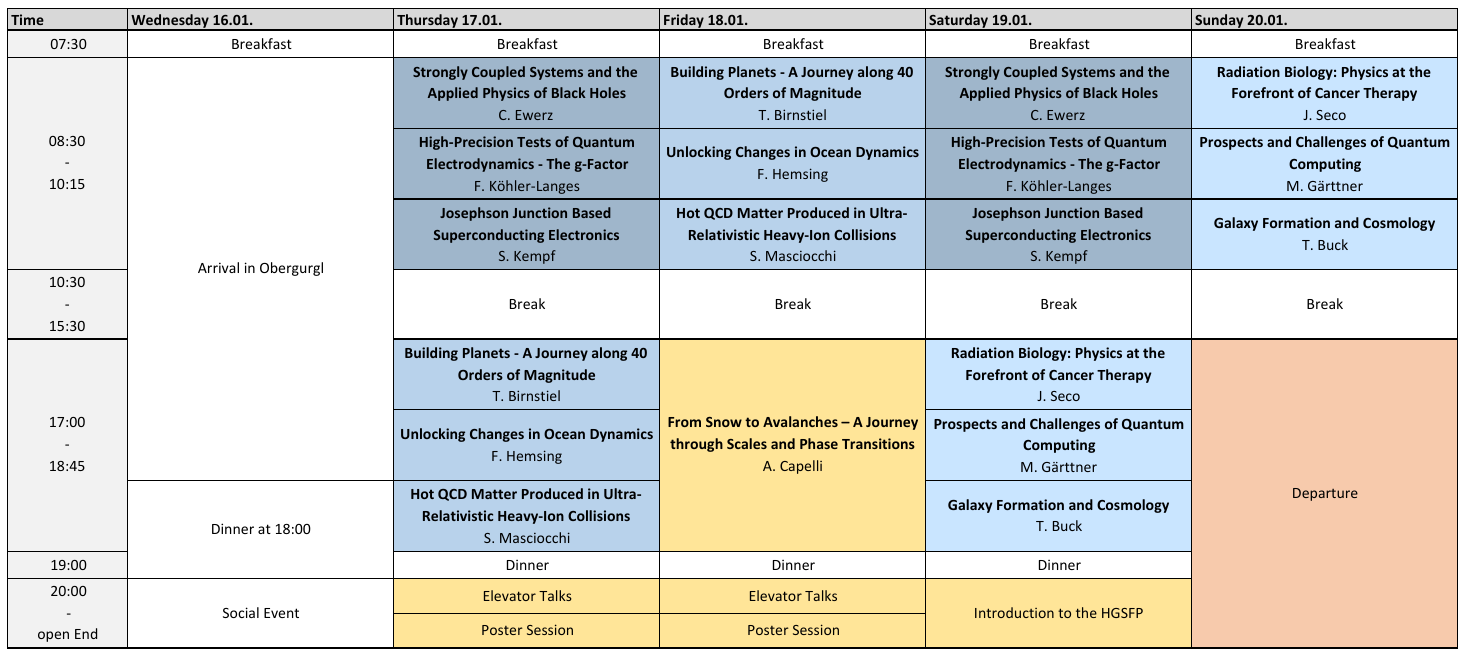
\includegraphics[scale=0.66, angle = 90 ]{figures/Program.jpg}
\end{figure}

\newpage